\documentclass[nooutcomes]{ximera}
\usepackage{gensymb}
\usepackage{tabularx}
\usepackage{mdframed}
\usepackage{pdfpages}
%\usepackage{chngcntr}

\let\problem\relax
\let\endproblem\relax

\newcommand{\property}[2]{#1#2}




\newtheoremstyle{SlantTheorem}{\topsep}{\fill}%%% space between body and thm
 {\slshape}                      %%% Thm body font
 {}                              %%% Indent amount (empty = no indent)
 {\bfseries\sffamily}            %%% Thm head font
 {}                              %%% Punctuation after thm head
 {3ex}                           %%% Space after thm head
 {\thmname{#1}\thmnumber{ #2}\thmnote{ \bfseries(#3)}} %%% Thm head spec
\theoremstyle{SlantTheorem}
\newtheorem{problem}{Problem}[]

%\counterwithin*{problem}{section}



%%%%%%%%%%%%%%%%%%%%%%%%%%%%Jenny's code%%%%%%%%%%%%%%%%%%%%

%%% Solution environment
%\newenvironment{solution}{
%\ifhandout\setbox0\vbox\bgroup\else
%\begin{trivlist}\item[\hskip \labelsep\small\itshape\bfseries Solution\hspace{2ex}]
%\par\noindent\upshape\small
%\fi}
%{\ifhandout\egroup\else
%\end{trivlist}
%\fi}
%
%
%%% instructorIntro environment
%\ifhandout
%\newenvironment{instructorIntro}[1][false]%
%{%
%\def\givenatend{\boolean{#1}}\ifthenelse{\boolean{#1}}{\begin{trivlist}\item}{\setbox0\vbox\bgroup}{}
%}
%{%
%\ifthenelse{\givenatend}{\end{trivlist}}{\egroup}{}
%}
%\else
%\newenvironment{instructorIntro}[1][false]%
%{%
%  \ifthenelse{\boolean{#1}}{\begin{trivlist}\item[\hskip \labelsep\bfseries Instructor Notes:\hspace{2ex}]}
%{\begin{trivlist}\item[\hskip \labelsep\bfseries Instructor Notes:\hspace{2ex}]}
%{}
%}
%% %% line at the bottom} 
%{\end{trivlist}\par\addvspace{.5ex}\nobreak\noindent\hung} 
%\fi
%
%


\let\instructorNotes\relax
\let\endinstructorNotes\relax
%%% instructorNotes environment
\ifhandout
\newenvironment{instructorNotes}[1][false]%
{%
\def\givenatend{\boolean{#1}}\ifthenelse{\boolean{#1}}{\begin{trivlist}\item}{\setbox0\vbox\bgroup}{}
}
{%
\ifthenelse{\givenatend}{\end{trivlist}}{\egroup}{}
}
\else
\newenvironment{instructorNotes}[1][false]%
{%
  \ifthenelse{\boolean{#1}}{\begin{trivlist}\item[\hskip \labelsep\bfseries {\Large Instructor Notes: \\} \hspace{\textwidth} ]}
{\begin{trivlist}\item[\hskip \labelsep\bfseries {\Large Instructor Notes: \\} \hspace{\textwidth} ]}
{}
}
{\end{trivlist}}
\fi


%% Suggested Timing
\newcommand{\timing}[1]{{\bf Suggested Timing: \hspace{2ex}} #1}




\hypersetup{
    colorlinks=true,       % false: boxed links; true: colored links
    linkcolor=blue,          % color of internal links (change box color with linkbordercolor)
    citecolor=green,        % color of links to bibliography
    filecolor=magenta,      % color of file links
    urlcolor=cyan           % color of external links
}

\title{Volume Problems}
\author{Vic Ferdinand, Betsy McNeal, Jenny Sheldon}

\begin{document}
\begin{abstract}
\end{abstract}

\maketitle



\begin{problem}
Find the volume of the following solid in two different ways.

\[
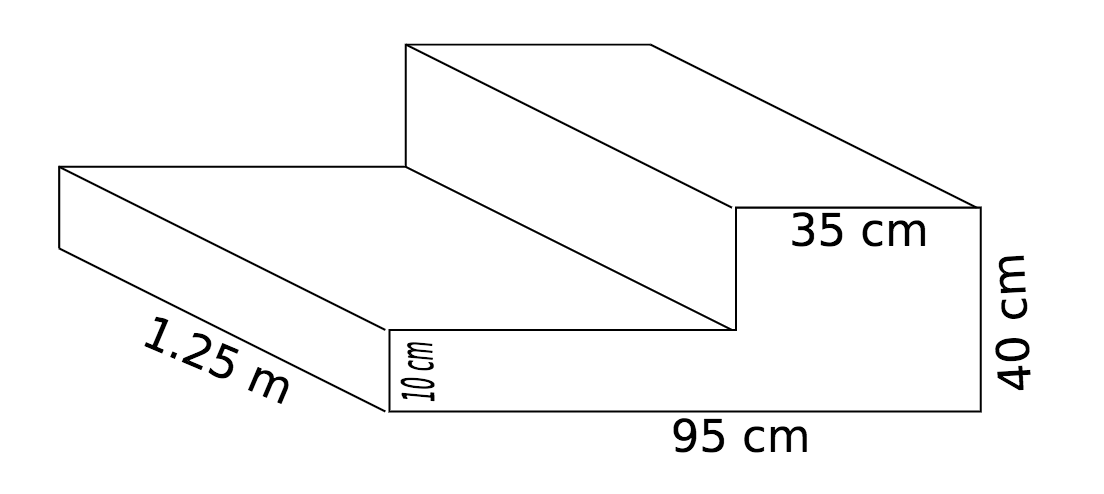
\includegraphics[height=1.5in]{elementaryActivities/graphics/prism-volume.png}
\]
\end{problem}

\begin{problem}
The figure depicts a quonset hut that will house temporary workers.  (You can google ``quonset hut'' if you've never heard of one!)  The front and back faces are semi-circular with a height of 12 feet, and the floor of the hut is a square.

\[
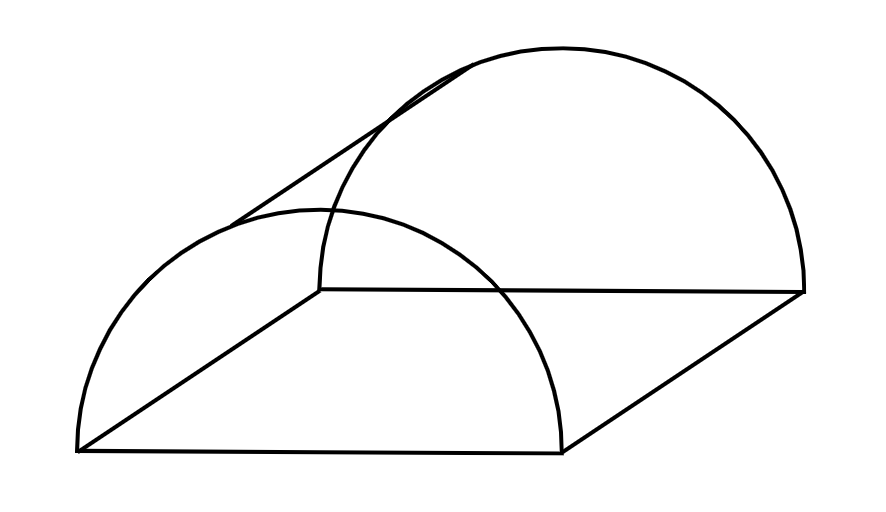
\includegraphics[height=1.5in]{elementaryActivities/graphics/quonsetHut.png}
\]

\begin{enumerate}
    \item Find the volume and surface area of the hut in two different ways (each).
    \item The ``roof'' of the hut will be constructed from steel which costs \$2.50 per square foot. The front and back will be constructed from steel which costs \$4 per square foot.  The ``floor'' of the hut will be constructed from wooden planks which cost \$1 per square yard. How much will it cost to build this hut?
\end{enumerate}
\end{problem}

\newpage
\begin{problem}
You are teaching a lesson about volume and surface area.
    \begin{itemize}
        \item Aly claims that the volume of a solid must always be less than the surface area of that solid, because the surface area holds in the volume.
        \item Simone claims that the volume of a solid must always be greater than the surface area of that solid, because the surface area is so thin.
    \end{itemize}
    Discuss the girls' ideas.  Is either of them completely correct?  How could you help each of the girls better understand the relationship between volume and surface area?
\end{problem}


\newpage
\begin{instructorNotes}
This activity is primarily intended to give students practice calculating volume flexibly.  The activity also contains some unit conversion issues, as well as consideration of surface area.  In our course, this is the first time students work to calculate volumes of irregular figures and the first time we work with both volume and surface area.  We have already worked with moving and additivity principles of volume, so our students find applying these principles with volume to be straightforward.  For us, this activity directly follows one about unit conversion with area and volume, and is the last activity we do on volume.

\begin{itemize}
    \item We see many creative ways of solving the first problem.  The most common are: cutting into two (or more) rectangular prisms, using the ``side'' as the base of the object, and fitting together two copies of the object to make a rectangular prism.
    \item The second problem tends to be fairly straightforward for our students, at least in terms of the volume.  The complication tends to be in calculating the surface area, especially if they haven't done this in some time, and in how many different calculations they need to do to arrive at their final answer. 
    \item We encourage students to work through the third problem by looking at examples.  We have frequently found that students need to be encouraged to work with fractional side lengths or other non-whole numbers.
    \item The third problem also brings up some dimensionality issues.  We have found that our students really struggle to identify the dimension of an object, and surface area is a particularly confusing example for them.  
    \item In our course, we have previously discussed a relationship between a fixed perimeter and the various areas that perimeter can enclose.  If we get a chance to work though this question, we point out that we could make similar arguments with surface area and volume.

\end{itemize}

\timing{We usually take the whole class period for this activity.  We give students 5-10 minutes to work in groups on the first problem, then take 15-20 minutes to discuss this problem.  The more different types of solutions we discuss, the longer this usually takes.  We then repeat the process for the second problem.  We don't usually get to the third problem in class.  We have found this to be a difficult question for students, and we typically don't have much time to spend on in-depth questions about surface area.  As a result, we have moved this idea (and this question) to one of our end-of-semester projects.}

\end{instructorNotes}




\end{document}